\chapter[Motor Control II: Learning the Swing]{Motor Control II:\\Learning the Swing}
\label{ch:motor_learning}
\raggedbottom
\index{visual attention}
\index{variability in practice}
\index{transfer of learning}
\index{temporal difference learning}
\index{setpoint hypothesis}
\index{sensory template}
\index{self-organization}
\index{schema theory}
\index{reinforcement learning}
\index{reference trajectory}
\index{random practice}
\index{quiet eye}
\index{proprioceptors}
\index{proprioception}
\index{practice design}
\index{neocortex}
\index{muscle spindles}
\index{motor schema}
\index{motor memory}
\index{motor learning}
\index{motor cortex}
\index{motor control}
\index{long-term depression}
\index{learning stages}
\index{learning rules}
\index{kinesthetic sensation}
\index{joint receptors}
\index{internal focus}
\index{individual differences}
\index{ideomotor theory}
\index{hierarchical processing}
\index{genetic factors}
\index{gaze fixation}
\index{feel}
\index{external focus}
\index{expertise}
\index{ecological dynamics}
\index{dynamical systems}
\index{dopamine}
\index{differential learning}
\index{deliberate practice}
\index{degrees of freedom}
\index{cortical hierarchy}
\index{contextual interference}
\index{constraints-led approach}
\index{cerebellum}
\index{cerebellar learning}
\index{blocked practice}
\index{basal ganglia}
\index{attractors}
\index{attentional focus}
\index{Golgi tendon organs}
\index{Fitts and Posner}
\index{DOF problem}
\index{Bernstein's problem}
\index{10,000-hour rule}

\begin{laymansbox}{What This Chapter Is About}{box:ch25_intro}
A well-struck shot leaves several kinds of information: the ball's flight, contact sound, pressure at the hands, effort, balance and the golfer's judgment of the result. Learning involves finding which information predicts useful outcomes, then changing preparation and action so those outcomes become more reliable. The sensation of a good swing can help, but reproducing a sensation does not guarantee reproducing its mechanics or result.

This chapter connects feel to physical state, prediction, task goals and practice design. Its central distinction is between performing well now and acquiring a capability that survives a delay or a change of conditions. Neither a satisfying shot nor a compelling explanation of it is sufficient evidence of lasting learning.
\end{laymansbox}

\section{Stages of Motor Learning}
\label{sec:ch25_stages}

Fitts and Posner's cognitive, associative and autonomous stages describe changing demands on attention and skill organization \citep{fitts1967human}. They are useful descriptions, not a fixed timetable, a neurological diagnosis or a guarantee that improvement proceeds monotonically. A golfer may execute a familiar putt automatically while deliberately learning an unfamiliar bunker shot.

\begin{definition}{Cognitive Stage}{ch25_cognitive}
The learner is establishing the task, relevant cues and possible actions. Instructions and explicit strategies may occupy substantial attention. What matters is the difficulty of organizing this task for this learner, not the number of weeks since a first lesson.
\end{definition}

\begin{definition}{Associative Stage}{ch25_associative}
The learner is refining relationships among preparation, action, feedback and results. Some components become reliable while others remain uncertain. Improvement can involve a better strategy, more accurate prediction, different coordination or better use of feedback.
\end{definition}

\begin{definition}{Autonomous Stage}{ch25_autonomous}
Execution demands less deliberate supervision in a familiar context. Automaticity does not mean perfect repetition, immunity to pressure or absence of neural feedback. A change of equipment, lie or task can require renewed attention.
\end{definition}

\begin{example}{The Three Stages in Golf}{ch25_stages_example}
Consider learning distance control in putting. Initially the golfer may consciously compare stroke size and roll distance. Later, a familiar distance can evoke an effective preparation without that calculation. To assess the change, record both distance error and the attention required. A single lower error does not establish a stage transition; fatigue, warm-up and helpful instructions can temporarily alter performance.
\end{example}

There is no justified one-to-one sequence from prefrontal cortex to premotor cortex to cerebellum. Behavioral stages do not identify the neural structures responsible for them. Likewise, variability need not fall in every joint as skill improves. We need a task-level account before deciding which variation is beneficial or harmful.

\subsection{Bernstein's Problem: Coordination and Task Redundancy}
\label{subsec:ch25_bernstein}

\begin{definition}{Bernstein's Problem}{ch25_bernstein_problem}
A body has many mechanically coupled degrees of freedom and many possible muscle actions. A task usually constrains only some combinations of these variables. The coordination problem is to organize feasible actions that achieve the task while respecting physical and physiological constraints \citep{bernstein1967coordination}.
\end{definition}

The number of degrees of freedom depends on the model: its joints, constraints, flexible structures and contact assumptions. Position, velocity and acceleration are not three independently selectable commands at every joint. They are related by differentiation and equations of motion. Muscle redundancy introduces another distinction: different activation patterns may produce similar net joint torques while differing in force, stiffness and metabolic demand.

\begin{principle}{Three Coordination Strategies}{box:ch25_bernstein_strategies}
Restricting joint motion, coupling motions and exploiting mechanical interactions are possible strategies. They are not obligatory beginner, intermediate and expert stages. Restricting motion can simplify a task but increase effort; allowing more motion can improve adaptability or make delivery less reliable. No strategy is most energy-efficient without a specified system, task and energy measure.
\end{principle}

\begin{example}{Bernstein's Problem in Golf}{ch25_bernstein_golf}
Suppose two small joint deviations contribute to a scalar delivery error as $y=q_1+q_2$. All pairs satisfying $q_2=-q_1$ cancel in this local task model. A golfer can vary both joints while preserving delivery. If a different club or operating point changes the sensitivity to $y=q_1+2q_2$, the same cancellation no longer works. A coordination pattern is task- and context-dependent.
\end{example}

More generally, let delivery be $\bm{y}=G(\bm{x},c)$, where $c$ specifies club, lie and other conditions. Near a nominal state, $\delta\bm{y}\approx J\delta\bm{x}$, with $J=\partial G/\partial\bm{x}$. For zero-mean deviations with covariance $\Sigma_x$,
\[
\Sigma_y\approx J\Sigma_xJ^{\mathsf T}.
\]
For a scalar output with mean error $\mu_y$, mean squared task error is $\mu_y^2+\operatorname{Var}(y)$. Precision and bias must both be assessed. If $\bm{x}$ mixes angles, velocities and forces, its covariance has mixed units; a raw trace is not a coordinate-independent measure of skill.

Even with two identically scaled angular coordinates, smaller joint variability can mean greater task variability. For $J=(1,1)$, consider manufactured covariance matrices in squared degrees:
\[
\Sigma_A=\begin{pmatrix}1&0.9\\0.9&1\end{pmatrix},\qquad
\Sigma_B=\begin{pmatrix}4&-3.8\\-3.8&4\end{pmatrix}.
\]
Both are positive definite. Although $\operatorname{tr}\Sigma_A=2<8=\operatorname{tr}\Sigma_B$, the task variances are $3.8$ and $0.4$ square degrees respectively. The second pattern has greater joint variation but better cancellation. This proves a limitation of a variability metric, not that a particular golfer uses a neural synergy. Measurement error, shared mechanics and task constraints can also produce covariance.

\begin{figure}[H]
\centering
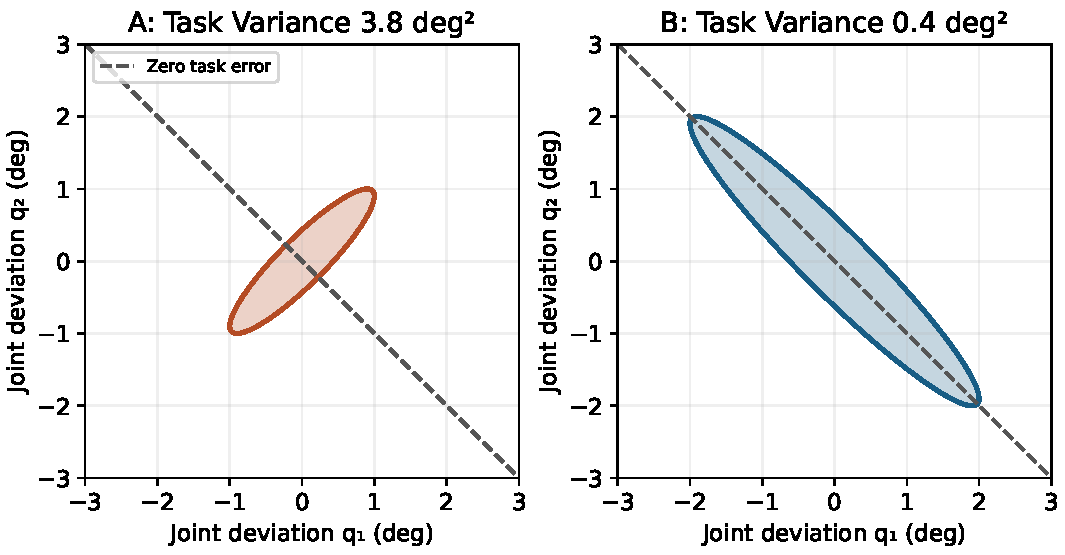
\includegraphics[width=\linewidth]{figures/motor_learning_covariance.pdf}
\caption{Manufactured Covariance Ellipses for the Task $y=q_1+q_2$. Greater Joint Variation Can Coexist With Smaller Task Variance. Ellipses Have Unit Mahalanobis Radius; They Are Not Human Measurements.}
\label{fig:ch25_coordination_covariance}
\end{figure}

\section{The Feel of a Good Shot: Proprioception as a Control Cue}
\label{sec:ch25_feel_good_shot}

\begin{principle}{The Setpoint Hypothesis: Feel as a Testable Cue}{ch25_setpoint_hypothesis}
A remembered sensation may serve as a cue for preparing or evaluating a swing. Calling it a reference or setpoint is a modeling choice. The hypothesis becomes useful when it predicts observable changes under altered sensory feedback or task conditions. It does not establish that the nervous system stores and replays one complete sensory trajectory.
\end{principle}

\subsection{Proprioception: Signals and State Estimates}
\label{subsec:ch25_proprioception}

\begin{principle}{Proprioceptive Receptors}{box:ch25_proprioceptors}
Muscle spindle, tendon, skin and joint afferents contribute information related to movement, position and force. Their signals depend on physiological and mechanical conditions. Perception combines populations of signals with central information; there is no single receptor that directly reports a perfectly calibrated joint angle or total muscle force \citep{proske2012proprioceptive}.
\end{principle}

The golfer's report of feel also includes touch, vision, sound, effort and vestibular information. Vestibular signals concern head motion and orientation, including angular motion and gravito-inertial acceleration; they are not equivalent to eye position. Holding the gaze near the ball does not establish a stationary head or silence vestibular input. A joint's perceptual accuracy cannot be assigned a universal threshold independently of movement, load and measurement protocol.

Let the physical state include configuration $\bm{q}$, velocity $\bm{v}$, activation $\bm{a}$ and relevant elastic or contact states $\bm{z}$:
\[
\bm{x}=(\bm{q},\bm{v},\bm{a},\bm{z}),\qquad
\dot{\bm{x}}=f(\bm{x},\bm{u},c).
\]
An illustrative sensory channel is
\[
\bm{s}_t=h(\bm{x}_{t-d},c)+\bm{\eta}_t.
\]
Here $d$ is that channel's delay and $\bm{\eta}_t$ represents noise or unmodeled influences. An estimator combines observations, command history and a forward model to form $\hat{\bm{x}}_t$. Neither the observer nor the golfer is thereby granted direct access to the complete physical state. Different channels have different delays and reliabilities; treating them as one synchronous measurement can create apparent prediction errors.

An elementary Gaussian example clarifies the role of reliability. Suppose an unbiased scalar prediction is $20^\circ$ with variance $9\,\mathrm{deg}^2$, and an independent unbiased observation is $22^\circ$ with noise variance $1\,\mathrm{deg}^2$. Combining their precisions gives an estimate of $21.8^\circ$ and variance $0.9\,\mathrm{deg}^2$. This is a calculation under stated assumptions, not an asserted neural algorithm. If the prediction and observation share an error, the independence assumption fails and confidence can be overstated.

\subsection{Reference Trajectories, Predictions and Policies}
\label{subsec:ch25_reference_trajectory}

\begin{constraintbox}{Pedagogical Simplification}{box:ch25_simplification}
A desired trajectory, a predicted trajectory and an estimated trajectory answer different questions: what should happen, what is expected to happen, and what appears to be happening. A successful controller need not make all three identical. A reference trajectory is one possible representation; a policy can choose actions from estimated state, task and context without replaying one fixed path.
\end{constraintbox}

Write a policy as $\bm{u}_t=\pi_\theta(\hat{\bm{x}}_t,c,g,t)$, with goal $g$ and adjustable parameters $\theta$. Learning may change the estimator, the policy, the valuation of outcomes or the preparation of the initial state. A familiar feeling can cue a policy without uniquely specifying its mechanical trajectory. The same verbal description of feel can accompany different motions; similar motions can feel different when fatigue or sensory conditions change.

\begin{example}{The Feel of a Good Swing}{ch25_feel_example}
A golfer reports a light grip and an unhurried transition after a centered strike. Record the report alongside impact location, delivery and ball flight. If the cue predicts centered contact across later trials and relevant conditions, it has practical value. If the player reports the same feel while contact moves across the face, the cue needs recalibration. Neither result requires dismissing subjective experience or treating it as an instrument reading.
\end{example}

Impact sensations mostly inform evaluation and later attempts. A response triggered by the collision cannot causally correct an earlier impact condition. Forces and vibrations measured at the clubhead cannot be equated to loads throughout the body without a transmission model. A prepared grip or muscle state may affect impact mechanically; that differs from a new neural correction initiated after contact. The computational-brain and impact chapters treat those timing and coupling questions separately.

\section{Contemporary Motor Learning Frameworks}
\label{sec:ch25_learning_frameworks}

Frameworks emphasize different explanatory levels: generalization across tasks, relations between a performer and environment, coordination dynamics, or changes induced by varied practice. Their terminology does not make them mutually exclusive, and a successful drill rarely identifies one uniquely correct theory.

\begin{samepage}
\subsection{Schema Theory}
\label{subsec:ch25_schema}

\begin{definition}[unbreakable]{Motor Schema}{ch25_schema}
In schema theory, experience supports relationships among initial conditions, response specifications, sensory consequences and outcomes, allowing a skill to be parameterized for new requirements \citep{schmidt1975schema}. This is a theoretical account of generalization, not a claim that distance is converted into force by one universal linear rule.
\end{definition}
\end{samepage}

\begin{example}{Golf Schema}{ch25_golf_schema}
For a projectile launched and landing at equal height in a vacuum, $R=v_0^2\sin(2\alpha)/g$. At fixed angle $\alpha$ with positive $\sin(2\alpha)$, $v_0$ scales as $\sqrt{R}$: quadrupling range doubles launch speed. Real golf adds aerodynamic forces, spin, unequal elevations and ground interaction. Even this simplified case disproves a universal proportionality between required speed and distance. Launch speed also does not uniquely determine a muscle-force history.
\end{example}

Practicing several distances can supply information about a response-to-outcome relationship. Whether that information transfers depends on where practice samples the relationship, how noisy the feedback is and whether test conditions preserve it. Interpolating among familiar distances and extrapolating to a different club or lie are different problems. A theory's prediction of useful variation is not proof that every varied schedule beats every constant schedule.

\subsection{Ecological Dynamics and Constraints-Led Approach}
\label{subsec:ch25_ecological}

\begin{definition}{Ecological Dynamics}{ch25_ecological_dynamics}
An approach that studies action in relation to the performer, task and environment, emphasizing how information and available opportunities for action shape coordination \citep{davids2008dynamics}.
\end{definition}

\begin{definition}{Constraints-Led Approach}{ch25_constraints_led}
Practice design that changes task, environmental or performer-related constraints to encourage exploration of useful solutions. Examples include target size, lie, club and permitted landing area. The resulting solution must be measured; the constraint does not uniquely prescribe it.
\end{definition}

A shorter target may change backswing amplitude, speed, launch or club choice. It does not force energy transfer to occur earlier. A narrow corridor penalizes dispersion but does not mechanically require a draw. The design question is whether the drill makes the intended information and skill relevant while retaining a meaningful relationship to the eventual golf task. A drill can be difficult yet teach an adjustment that does not transfer.

\subsection{Dynamical Systems Theory and Attractors}
\label{subsec:ch25_dynamical_systems}

\begin{definition}{Movement Attractor}{ch25_attractor}
An attractor is an invariant set approached by trajectories from a specified neighborhood in a specified dynamical system. A finite swing that ends at impact is not automatically an attractor. One may instead study finite-time sensitivity, a time-dependent tracking system, or a return map across repeated trials, stating the system and stability definition \citep{kelso1995dynamic}.
\end{definition}

\begin{example}{Attractors in Golf}{ch25_attractors}
For a deliberately simplified trial model, let $m_n$ be a learned scalar response and let $r$ be a fixed required response. Set
\[
m_{n+1}=a m_n+b(r-m_n).
\]
The retention factor $a$ and error sensitivity $b$ are dimensionless model parameters, not measured neural constants. For $a=1$, the task error $e_n=r-m_n$ satisfies $e_{n+1}=(1-b)e_n$. With $r=4$ and $m_0=0$, $b=0.25$ gives errors $4,3,2.25,1.6875,\ldots$. With $b=1.5$, errors alternate in sign while shrinking. With $b=2.1$, their magnitude grows. More aggressive correction can destabilize this model.
\end{example}

The general stability condition is $|a-b|<1$. When stable and $1-a+b\ne0$, the equilibrium is $m_*=br/(1-a+b)$, leaving error $e_*=(1-a)r/(1-a+b)$. For $a=0.98$, $b=0.25$ and $r=4$, this error is $8/27\approx0.2963$. These equations separate stability from zero error and immediate change from retention. They are manufactured examples, not fitted rates of golf learning or proof of a particular practice schedule.

\begin{figure}[H]
\centering
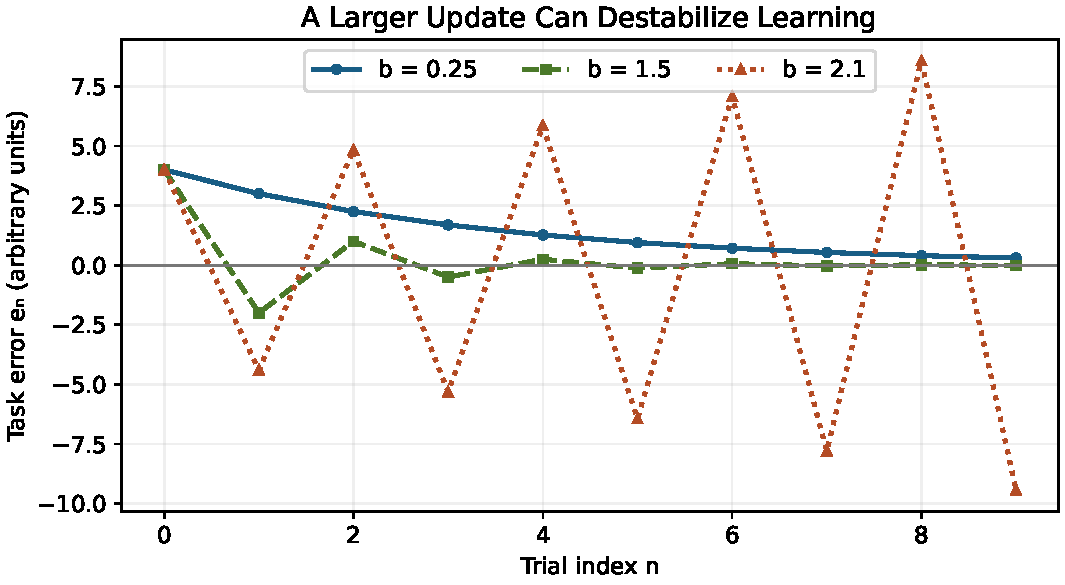
\includegraphics[width=\linewidth]{figures/motor_learning_updates.pdf}
\caption{Manufactured Trial Updates With $a=1$, $r=4$ and $m_0=0$. Gains of 0.25 and 1.5 Converge; a Gain of 2.1 Diverges. These Curves Do Not Represent Measured Learning Stages.}
\label{fig:ch25_learning_stages}
\end{figure}

\subsection{Differential Learning and Noise}
\label{subsec:ch25_differential}

\begin{definition}{Differential Learning}{ch25_differential}
Wolfgang Immanuel Sch\"ollhorn's differential-learning approach deliberately varies movement conditions and emphasizes fluctuations during practice. It is conceptually distinct from merely randomizing the order of several practiced tasks \citep{schollhorn2016commentary}.
\end{definition}

\begin{example}{Differential Learning in Golf}{ch25_differential_golf}
Varying stance or stroke conditions introduces movement variation. Randomizing three target distances changes task order. Repeating one distance in blocks changes neither in the same way. A useful comparison specifies the actual manipulations, total attempts, feedback and later test. Calling a drill differential, variable or random does not establish its effectiveness.
\end{example}

Variation can reveal a useful relationship or obscure it. For example, changing stance, club, target and feedback together makes it difficult to attribute an improvement to one element. This does not forbid combined practice; it limits what that practice can establish scientifically. Added noise is not intrinsically beneficial, and its amplitude and relevance matter.

\section{Neural Networks in the Brain: What the Evidence Establishes}
\label{sec:ch25_neural_networks}

\subsection{The Neocortex: Distributed Learning}
\label{subsec:ch25_neocortex}

\begin{principle}{The Cortical Hierarchy for Motor Control}{box:ch25_cortical_hierarchy}
Planning, perception and action involve interacting cortical and subcortical systems. A hierarchical diagram can organize computational roles, but arrows in that diagram are not evidence for a literal serial pipeline. Behavioral adaptation, explicit strategy, reinforcement and skill acquisition need to be distinguished before assigning a mechanism \citep{kitago2013motor}.
\end{principle}

An observation that two regions are active during learning does not establish which computed the error, which changed a command or where a memory is stored. Those claims require experiments that distinguish the alternatives. Golf adds a further generalization step: a result from a laboratory pointing task may motivate a golf hypothesis without validating it.

\subsection{The Cerebellum: Plasticity and Prediction}
\label{subsec:ch25_cerebellum_learning}

\begin{principle}{Cerebellar Learning Mechanism}{box:ch25_cerebellar_learning}
One influential account involves long-term depression at parallel-fiber--Purkinje-cell synapses, with climbing-fiber activity contributing to plasticity induction. It is not a synapse between parallel and climbing fibers. Nor is that plasticity the only possible learning mechanism. Schonewille and colleagues found preserved performance on several motor-learning tasks in three mouse lines with disrupted expression of this form of LTD. The result limits an obligatory single-mechanism account; it does not establish that LTD is irrelevant in all tasks or species \citep{schonewille2011ltd}.
\end{principle}

A useful mathematical teaching model is gradient learning of a prediction. Let a scalar predicted observation be $\hat s_n=\bm{w}_n^{\mathsf T}\bm{\phi}_n$ with loss $L_n=\tfrac12(s_n-\hat s_n)^2$. Then
\begin{equation}
\bm{w}_{n+1}=\bm{w}_n+\eta(s_n-\hat s_n)\bm{\phi}_n.
\label{eq:ch25_ltd_rule}
\end{equation}
This follows by differentiating the specified quadratic loss. The sign depends on defining error as observed minus predicted. It is not an experimentally established synaptic law for golf. Features, timing, learning rate and biological implementation are additional hypotheses.

\subsection{The Basal Ganglia: Reinforcement Learning}
\label{subsec:ch25_basal_ganglia_learning}

\begin{principle}{Dopamine and Reward Prediction Error}{box:ch25_dopamine}
Schultz, Dayan and Montague related phasic dopamine responses in conditioning experiments to reward prediction error. A predicted reward need not produce the phasic increase elicited by an unexpected reward; omission can produce a decrease relative to baseline. Their temporal-difference account is a computational interpretation, not a claim that every dopamine neuron reports only one scalar or that a successful golf shot stores its entire trajectory \citep{schultz1997dopamine}.
\end{principle}

Using time index $t$ within an episode, a standard temporal-difference expression is
\[
\delta_t=R_{t+1}+\gamma V(\chi_{t+1})-V(\chi_t),\qquad 0\leq\gamma\leq1.
\]
Here $\chi_t$ denotes the model's informational state; $V$ predicts discounted future reward and $R$ is a scalar reward in the model. A complete episode or discounting assumption is required for the return to be well-defined. At a terminal state $V(\chi_{t+1})=0$. A reward of $1$ expected with value $1$ gives $\delta=0$; the same reward expected with value $0.25$ gives $0.75$. Zero error is not zero reward or absence of baseline neural firing.

Reward design matters. A practice score that rewards carry alone may favor a different behavior from one that penalizes missed fairways or poor contact. A scalar outcome also leaves a credit-assignment problem: which preparation, timing or command helped? It does not directly identify a vector of muscle corrections. Explicit reasoning, structured exploration and sensory information can all help distinguish candidate changes.

\section{The Setpoint Hypothesis: Errors and Testable Predictions}
\label{sec:ch25_setpoint_mechanism}

\begin{principle}{The Setpoint Hypothesis: A Mechanistic Model to Test}{ch25_setpoint_mechanism}
\label{thm:ch25_setpoint}
Suppose a golfer uses a remembered sensory pattern to help prepare a policy and evaluate its execution. This model should be tested against alternatives in which task outcomes, explicit aiming or other sensory cues dominate. Successful prediction in one context does not establish a unique stored pattern, its anatomical location or a universal explanation of swing failure.
\end{principle}

Four errors clarify what such a test must measure:
\begin{enumerate}
\item Tracking error compares a specified desired state with an estimate: $\bm{e}_{\mathrm{track}}=\bm{x}_{\mathrm{ref}}-\hat{\bm{x}}$. The reference must be defined in compatible coordinates and at a compatible time.
\item Sensory prediction error compares an observation with the predicted observation: $\bm{e}_{\mathrm{sens}}=\bm{s}-\hat{\bm{s}}^-$. Predictions must account for the channel's delay. This is not desired minus actual state.
\item Task error compares the desired and observed outcome: $\bm{e}_{\mathrm{task}}=\bm{y}_{\mathrm{goal}}-\bm{y}_{\mathrm{obs}}$. It depends on the chosen task, such as landing location rather than a joint angle.
\item Reward prediction error compares received and subsequently predicted value with previous expected value. It is not the task-error vector or a synonym for disappointment.
\end{enumerate}

These quantities can disagree. In a manufactured pointing example, a hand at $-45^\circ$ with a $+45^\circ$ displayed rotation places a cursor on a $0^\circ$ target. Task error is zero. If the predicted cursor is still $-45^\circ$, sensory prediction error is $+45^\circ$. Mazzoni and Krakauer's visuomotor experiment provides a related empirical dissociation: an explicit compensatory strategy initially achieved the task, yet subsequent implicit adaptation caused drift away from it \citep{Mazzoni2006Strategy}. That result concerns the tested pointing perturbation, not an inevitability that explicit golf instruction must fail.

\begin{example}{What the Setpoint Hypothesis Can Predict}{ch25_setpoint_explains}
Before revealing ball-flight feedback, ask the player to rate expected contact and direction. Then compare the prediction with measured contact and delivery. Separately record the felt movement and the actual outcome. Alter one relevant sensory or mechanical condition in a controlled comparison. If feel remains constant while delivery changes, a fixed-feel target is insufficient in that condition. If calibration improves, test whether it survives a delay and transfers. Expectation, attention and feedback changes remain competing explanations unless the design separates them.
\end{example}

A useful protocol therefore records predictions before outcomes, avoids selecting only memorable good shots and includes unsuccessful attempts. Otherwise hindsight can make a vague sensation appear more predictive than it was. Asking about feel may itself change attention, so compare equivalent questioning across conditions.

The model also does not diagnose the yips as a corrupted reference trajectory. Involuntary movements, anxiety-related performance changes and other clinical presentations require appropriate distinctions; the observational yips literature does not support a single universal cause \citep{Adler2011Yips}. Likewise, a return of an old swing under pressure does not prove that two stored trajectories were activated simultaneously. Describe the observed change first, then test explanations.

\section{Practice Design: Implications for Learning}
\label{sec:ch25_practice_design}

Practice performance is measured while training. Retention assesses the learned task after a delay, with the test conditions specified. Transfer assesses performance under a changed task or context. These are related but different outcomes. Temporary guidance, warm-up, fatigue and familiarity can change immediate performance without the same change in retained capability.

For illustration, suppose practice condition A ends with mean error $2$ and B with $3$ in the same units. On a matched delayed test A has error $6$ and B $4$. A looked better during acquisition; B is better on that retention test. These invented numbers demonstrate the logic of the comparison. They are not evidence for a particular drill, neural process or schedule. A test with the guidance removed also evaluates dependence on that guidance; report the change explicitly.

\subsection{Random vs. Blocked Practice: Contextual Interference}
\label{subsec:ch25_random_vs_blocked}

\begin{definition}{Blocked Practice}{ch25_blocked}
Repeated attempts at one task variant before switching to another, such as a block of putts at each of three distances.
\end{definition}

\begin{definition}{Random Practice}{ch25_random}
Task variants interleaved in an unpredictable order. The task set, number of attempts and feedback can be held constant while order changes.
\end{definition}

\begin{constraintbox}{Contextual Interference Depends on the Task}{box:ch25_contextual_interference}
Contextual interference concerns how mixing practiced tasks affects acquisition, retention and transfer. It is not a universal random-practice advantage. In Porter and Magill's novice putting experiment, a schedule progressing from blocked to serial to random practice produced better retention than the compared blocked and random schedules \citep{porter2010interference}. The result supports testing progression; it does not provide a universal dose for every golfer or full swing.
\end{constraintbox}

A practical design can start with enough repetition to understand the task and feedback, then introduce decisions representative of play. The transition should follow observed readiness and the purpose of practice, not a rule that difficulty is always desirable. Compare schedules with equal task exposure; otherwise increased variation, extra attempts or different feedback can explain the result.

\subsection{External vs. Internal Focus of Attention}
\label{subsec:ch25_focus}

\begin{definition}{Internal Focus}{ch25_internal_focus}
Attention directed toward the performer's body movement, such as the action of the arms.
\end{definition}

\begin{definition}{External Focus}{ch25_external_focus}
Attention directed toward an effect of movement, such as the club's motion or the intended ball flight. A cue such as ``smooth tempo'' is not inherently external; its meaning and the player's interpretation matter.
\end{definition}

Wulf, Lauterbach and Toole tested 22 golf novices practicing pitch shots. Attention to club motion, compared with arm motion, benefited practice and next-day retention without the instructions \citep{wulf1999golf}. This provides golf-specific evidence for that comparison. It does not show that all technical explanations impair learning, that every external cue is equivalent, or that one neurological mechanism has been uniquely established.

Technical analysis and an execution cue serve different purposes. Between attempts, a player and coach can use mechanics to diagnose delivery. During an attempt, a concise cue can direct attention toward the intended effect. Evaluate both the outcome and whether the cue is understood. The best-looking explanation is not necessarily the most useful instruction at the moment of execution.

\subsection{The Quiet Eye: Attention Timing}
\label{subsec:ch25_quiet_eye}

\begin{definition}{Quiet Eye}{ch25_quiet_eye}
A final task-relevant fixation or tracking gaze defined relative to a movement event, using explicit spatial and duration thresholds. It is an operational eye-tracking measure; the definition and relevant event must be reported for the task.
\end{definition}

Vine, Moore and Wilson studied 22 skilled male golfers in a putting intervention combining gaze feedback and instructions. The trained group improved some laboratory and competitive measures. Retention differences were not significant for every endpoint, and gaze data from five trained participants were lost. The authors also identified possible motivational confounding and limitations of putts per round as a putting measure \citep{vine2011competitive}. These results justify a bounded putting hypothesis, not a prescribed two-to-three-second fixation for every golf shot.

Gaze timing can influence information pickup, preparation and attention, but those are distinguishable candidate mechanisms. A relation between fixation duration and success does not establish how much success was caused by fixation. Extending a putting result to a driver requires a new argument and evidence. Eye stillness alone is not a measure of balance, head stability or vestibular activity.

\subsection{Deliberate Practice}
\label{subsec:ch25_deliberate_practice}

\begin{principle}{Characteristics of Deliberate Practice}{box:ch25_deliberate_practice}
For the practice plan here, specify the skill, a measurable criterion, feedback that can inform a change, a manageable challenge and a later test. This is an explicit design proposal, not a claim that every useful learning event requires immediate feedback or continuous conscious attention. Feedback frequency, timing and content are experimental choices.
\end{principle}

\begin{example}{Deliberate Practice in Golf}{ch25_deliberate_example}
For driver practice, choose a delivery-and-dispersion objective rather than maximum speed alone. Record club, ball, target, wind and measurement method. Obtain a baseline sample, test one defined cue or drill, and record every attempt under a stated inclusion rule. Later, repeat a matched assessment without extra coaching. Add a separate transfer test with another target or relevant condition. Report speed, strike location and dispersion together so improvement in one does not conceal deterioration in another.
\end{example}

Small samples deserve modest conclusions. Under an illustrative independent Bernoulli model, eight successes in ten attempts give an observed rate of $0.8$, but a 95\% Wilson interval is approximately $[0.490,0.943]$. Correlated attempts or changing conditions undermine that simple model. A single excellent shot provides still less information about reliability. Report uncertainty and the practical size of a change, not just whether a preferred cue produced one memorable result.

There is no arithmetic route from a large practice total to guaranteed expertise. At 52 weeks per year, 10 hours weekly for 10 years is 5,200 hours. Reaching 10,000 hours at that rate takes about 19.23 years; at 20 hours weekly it takes about 9.62 years. These are bookkeeping examples, not thresholds or recommended workloads. Practice histories differ in content, opportunity, feedback and recovery, so hours alone cannot identify the cause of different outcomes.

\section{Individual Differences: Why Learning Rates Differ}
\label{sec:ch25_individual_differences}

\begin{principle}{Sources of Individual Differences}{box:ch25_individual_diffs}
Prior experience, physical capabilities, sensory information, task understanding, practice opportunity, feedback and changing circumstances are candidate contributors to different learning trajectories. Observing a faster learner does not isolate a genetic, motivational or cognitive cause. Specify the comparison and consider baseline ability, task difficulty and measurement uncertainty.
\end{principle}

Transfer from another sport may involve perception, timing, physical capacity or useful strategies, but can also involve interference. Similarity of an action's appearance is insufficient: the relevant dynamics, equipment and success criterion may differ. Test what carries over under a defined change rather than assuming that ``athleticism'' explains every difference.

The affine-control viewpoint contributes a precise question: what must the golfer learn about how state, passive mechanics and commands jointly affect delivery? In a model $\dot{\bm{x}}=\bm{f}(\bm{x})+B(\bm{x})\bm{u}$, passive evolution is state-dependent, and the selected definition of zero input matters. A prepared activation or elastic state can remain after subsequent commands are set to zero. Learning may improve preparation or the timing of intervention; that does not make mechanics irrelevant or prove a unique energy-optimal strategy.

To test this connection, compare specified policies or counterfactual interventions from matched initial states and report feasible actuation, contact and uncertainty. Distinguish model prediction from human validation. A reduction in simulated commanded torque is not automatically lower muscular effort, lower joint loading or better transfer to play.

\begin{principle}{Key Takeaways}{box:ch25_takeaways}
Feel, mechanics and outcome provide related but nonidentical information. State estimates, desired trajectories, sensory predictions and reward predictions must be kept distinct. Coordination is judged against a task, including bias and covariance, rather than the smallest movement variation. Practice designs should make their proposed mechanism testable and assess retention and transfer. Neural and golf-specific claims must stay within the evidence that supports them.
\end{principle}

\begin{exercises}{Chapter Exercises}{ex:ch25_exercises}
\begin{enumerate}
\item Describe a golf skill you are learning. What observations distinguish increasing automaticity from a temporary reduction in task error?
\item After a poor shot, distinguish a useful report of feel from an inferred physical cause. Design one comparison that can test whether the report predicts contact quality.
\item Derive the speed ratio for vacuum ranges $R$ and $4R$ at fixed launch angle and equal launch/landing heights. Explain why it is not a force-scaling rule for golf.
\item Explain how a schedule can look better during practice but worse in retention. Identify two design differences that would confound a comparison of blocked and random practice.
\item Separate a mechanical diagnosis between attempts from an attentional cue during execution. What evidence would justify retaining the cue?
\item Define a quiet-eye measurement and explain why a putting intervention does not establish a universal full-swing fixation duration or a vestibular mechanism.
\item Design a progression from repetition to varied decisions for a beginner. Specify a criterion for advancing and a delayed test that could reveal dependence on guidance.
\item Calculate task variance for $J=(1,1)$ and the two covariance matrices in this chapter. Which coordination is more task-precise? Can the result rank muscular energy cost?
\item Derive the quadratic-loss prediction update. Explain the distinction between this algorithm and a demonstrated cerebellar synaptic mechanism.
\item Design a driver practice assessment with baseline, feedback, retention and transfer. Explain what eight successes in ten independent trials can and cannot establish.
\item For the scalar trial update, derive the stability condition and steady error. Relate preparation and model learning to the zero-input counterfactual without equating zero commands with zero activation.
\item Give an example of possible positive or negative transfer from another sport. Identify what must remain comparable and what must be measured before attributing the change to transfer.
\end{enumerate}
\end{exercises}

\section{Worked Answers}
\begin{enumerate}
\item Record task error over repeated, comparable assessments and how much deliberate supervision is required. A familiar task becoming easier to execute while preserving performance is compatible with automaticity. One warm-up improvement or helpful instruction cannot establish lasting change; add a delayed assessment.
\item Record a prediction of contact before seeing measured impact location, using the same questions in each condition. Compare all trials, not only good ones. An association supports the report's predictive use; manipulating a cue or sensory condition with appropriate controls is needed for a stronger causal claim.
\item From $v_0=\sqrt{Rg/\sin(2\alpha)}$, $v_0(4R)/v_0(R)=2$. The assumptions exclude golf aerodynamics and ground interaction. Mapping launch speed to force requires mass, impulse, coupling and a time history; distance alone does not provide these.
\item Temporary guidance can improve acquisition while a different condition retains more when guidance is removed. Unequal task exposure and different feedback confound an order comparison. Use matched delayed tests and state whether guidance, task order or context changed.
\item Diagnose measured face delivery, path or strike between shots, then test an understandable cue aimed at the intended effect during execution. Retain it if its practically useful benefit persists under suitable later tests, while tracking other outcomes and uncertainty. A verbal category alone is not proof of effectiveness.
\item Specify gaze location, allowable angular deviation, minimum duration and its timing relative to stroke events. The cited intervention concerns putting and bundles training elements. Neither outcome association nor eye fixation isolates head motion or vestibular processing.
\item Begin with repeated attempts that permit understanding feedback, then mix relevant distances or targets when the golfer can explain the task and respond meaningfully. Use a matched delayed test without extra prompts and a distinct transfer condition. The progression is a proposal to evaluate, not a universal optimum.
\item $J\Sigma_AJ^{\mathsf T}=1+1+2(0.9)=3.8$ and $J\Sigma_BJ^{\mathsf T}=4+4-2(3.8)=0.4$. B is more precise for this unbiased scalar task despite greater joint variation. Neither matrix supplies muscle work, activation or joint loading, so no energy ranking follows.
\item $\nabla_{\bm{w}}L=-(s-\bm{w}^{\mathsf T}\bm{\phi})\bm{\phi}$; subtracting $\eta\nabla L$ gives the stated update. Physiological interpretation additionally requires evidence for the features, teaching signal, timing, plasticity and task. A mathematical gradient is not evidence that those biological requirements hold.
\item Fix the target criterion and measurement conditions, record a baseline, compare a specified intervention, and repeat a delayed assessment plus a separate transfer test. The independent-trial Wilson interval for $8/10$ is approximately $[0.490,0.943]$. It shows substantial uncertainty; it does not establish an 80\% stable success probability or validity of independence.
\item Subtract the fixed point to get $m_{n+1}-m_*=(a-b)(m_n-m_*)$, so asymptotic stability requires $|a-b|<1$. Solving the fixed-point equation gives $e_*=(1-a)r/(1-a+b)$. Preparation changes the initial physical state; setting later commands to zero preserves that prepared state and is not necessarily zero torque or zero muscle force.
\item A prior sport might help target selection or timing but encourage an unsuitable equipment-specific motion. Compare relevant baseline skill and practice exposure, then assess the new task under controlled conditions. Shared joint motion alone cannot identify what transferred, and a failure to transfer is informative too.
\end{enumerate}
\clearpage
\flushbottom{}
